\chapter{模型视图教程}

每个 \hl{UI} 开发人员都应该了解模型视图编程,本教程的目的是让您轻松理解有关模型视图的相关知识。

表格,列表和树部件是 GUI 中经常使用的组件。这些部件可以通过两种不同的方式访问其数据。
传统方式是,这些部件包含用于存储数据的内部容器。这种方法非常直观,但是,在许多应用程序中,它会导致数据同步问题。
第二种方法是模型/视图编程,其中部件不维护内部数据容器。他们通过标准化接口访问外部数据,因此避免了数据重复。
乍一看,这似乎很复杂,但是如果您仔细看一看,不仅容易掌握,而且模型/视图编程的许多好处也变得更加明显。

\begin{figure}[hbt!]  
	% \centering
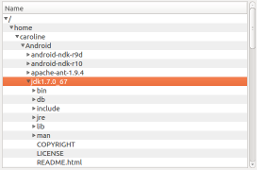
\includegraphics[width=0.3\textwidth]{treeview}
\end{figure}

在此过程中,我们将了解 \hl{Qt} 提供的一些基本技术,例如:

\begin{compactitem}
\item 标准部件和模型视图部件的区别
\item 窗体和模型之间的适配器
\item 开发一个简单的模型视图的应用程序
\item 预定义模型
\item 中间主题,比如:
\begin{compactitem}
\item 树形视图
\item 选项
\item 委托
\item 模型调试测试
\end{compactitem}
\end{compactitem}

您还将了解到新的应用程序是否可以通过模型/视图编程更容易地编写,或者经典的标准部件是否也可以工作。

本教程中的代码您可以编辑修改或者集成到您的项目中去。 
源码在 \hl{Qt} 的 \hl{examples/widgets/tutorials/modelview} 目录。

详见 参考文档

\section{介绍}

模型/视图是一种将数据从视图中分离出来,来处理数据集的一种技术。标准部件并不是为将数据从视图中分离出来而设计的,这就是为什么 Qt 会有两种不同类型的部件。
这两种部件看起来都一样,但是它们与数据之间的交互方式是不同的。

\begin{longtable}{|l|m{25em}|}
\hline
标准部件使用的数据最为部件的一部分。\\
&
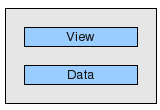
\includegraphics[width=0.4\textwidth]{standardwidget} \\ 
\hline	
视图类操作的是外部的数据(模型)。\\
&
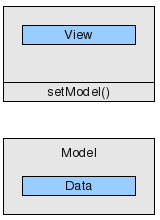
\includegraphics[width=0.4\textwidth]{modelview} \\ 
\hline	
\end{longtable}

\subsection{标准部件}

让我们仔细看一下标准表部件。表格部件是用户可以更改的数据元素的 2D 数组。
通过读取和写入表部件提供的数据元素,可以将表部件集成到程序流中。
该方法非常直观,在许多应用程序中很有用,但是使用标准表窗口部件显示和编辑数据库表可能会出现问题。
数据的两个副本必须协调一致:一个在部件外部;另一个在部件外部。开发人员负责同步两个版本。
除此之外,表示和数据的紧密耦合使编写单元测试更加困难。

\subsection{使用模型/视图解决}

模型/视图提供了一个使用更通用体系结构的解决方案。
模型/视图消除了标准控件可能出现的数据一致性问题。
模型/视图还可以更容易地使用同一数据的多个视图,因为一个模型可以传递给多个视图。
最重要的区别是模型/视图部件不在表单元格后面存储数据。实际上,它们直接根据您的数据进行操作。
因为视图类不知道数据的结构,所以需要提供一个包装器,使数据符合 QAbstractItemModel 接口。
视图使用此接口读取和写入数据。实现 QAbstractItemModel 类的任何实例都称为模型。
一旦视图接收到指向模型的指针,它将读取和显示其内容,并成为其编辑器。

\subsection{模型/视图部件概览}

下面是模型/视图部件及其对应的标准部件。

\begin{longtable}{|l|m{15em}|m{10em}|}
\hline
部件 & 标准部件 (基于项的便捷类) & 模型/视图 视图类 (使用外部数据) \\ 
\hline
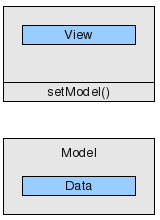
\includegraphics[width=0.4\textwidth]{modelview}  
&
QListWidget
&
QListView  \\
\hline
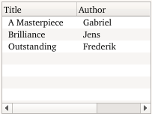
\includegraphics[width=0.4\textwidth]{tableview}  
&
QTableWidget	
&
QTableView \\
\hline
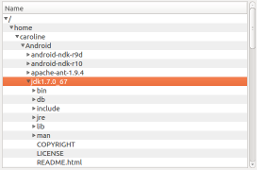
\includegraphics[width=0.4\textwidth]{treeview}  
&
QTreeWidget	
&
QTreeView  \\
\hline
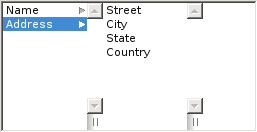
\includegraphics[width=0.4\textwidth]{columnview}  
&

&
QColumnView s显示列表层次结构的树视图  \\
\hline

\includegraphics[width=0.4\textwidth]{modelview-combobox}  
&
QComboBox 既可以用作视图类,也可以用作传统部件
&
  \\
\hline
\end{longtable}



\subsection{在表单和模型之间使用适配器}

在表单和模型之间使用适配器非常方便。
我们可以直接从表内部编辑存储在表中的数据,但是在文本字段中编辑数据更为方便。
在对部件的一个数据而不是数据集操作时,模型/视图并没有提供对应的方法将数据和视图分离开。
比如 QLineEdit,QCheckBox...因此我们需要一个适配器来将表单连接到数据源。

QDataWidgetMapper 是一个很好的解决方案,因为它可以将表单部件映射到表行,并且为数据库表构建表单非常容易。

\begin{figure}[hbt!]  
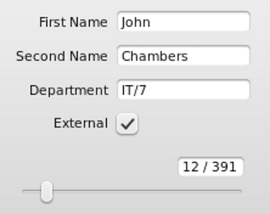
\includegraphics[width=0.3\textwidth]{widgetmapper}
\end{figure}

适配器的另一个例子是 QCompleter。
Qt 使用 QCompleter 在 Qt 部件(如 QComboBox 和 如下图所示的 QLineEdit)中提供自动补全功能。
QCompleter使用模型作为其数据源。
	
\begin{figure}[hbt!]  
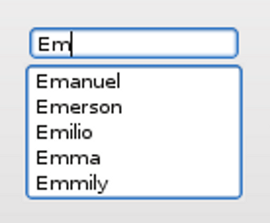
\includegraphics[width=0.3\textwidth]{qcompleter}
\end{figure}

\section{一个简单的模型/视图应用程序}

如果要开发模型/视图应用程序,应该从哪里开始?我们建议从一个简单的示例开始,并逐步扩展它。
这样更容易理解模型/视图架构。
事实证明,在调用 IDE 之前尝试详细了解模型/视图体系结构对于许多开发人员来说并不方便。
从具有演示数据的简单模型/视图应用程序开始要容易得多。
试试看!只需将以下示例中的数据替换为您自己的数据即可。

以下是7个非常简单和独立的应用程序,它们展示了模型/视图编程的不同方面。
可以在 examples/widgets/tutorials/modelview 目录中找到源代码。

\subsection{只读的表}

我们从使用 QTableView 来显示数据的应用程序开始。稍后我们将添加编辑功能。
(文件: examples/widgets/tutorials/modelview/1\_readonly/main.cpp)

\begin{cppcode}
// main.cpp
#include <QApplication>
#include <QTableView>
#include "mymodel.h"
	
int main(int argc, char *argv[])
{
	QApplication a(argc, argv);
	QTableView tableView;
	MyModel myModel;
	tableView.setModel(&myModel);
	tableView.show();
	return a.exec();
}
\end{cppcode}

main() 函数:

这是有趣的部分:我们创建 MyModel 的实例并使用 tableView.setModel(&myModel);。 
将其指针传递给 tableView。 tableView 将调用它收到的指针的方法来找出两件事:

\begin{compactitem}
\item 需要显示多少行和列。
\item 每个单元格中应该显示什么内容。
\end{compactitem}

模型需要一些代码来响应以上这些。

我们有一个表数据集,因此让我们从 QAbstractTableModel 开始,因为它比更通用的 QAbstractItemModel 更易于使用。

(文件:examples/widgets/tutorials/modelview/1\_readonly/mymodel.h)

\begin{cppcode}
// mymodel.h
#include <QAbstractTableModel>
	
class MyModel : public QAbstractTableModel
{
	Q_OBJECT
public:
	MyModel(QObject *parent = nullptr);
	int rowCount(const QModelIndex &parent = QModelIndex()) const override;
	int columnCount(const QModelIndex &parent = QModelIndex()) const override;
	QVariant data(const QModelIndex &index, int role = Qt::DisplayRole) const override;
};
\end{cppcode}

QAbstractTableModel 需要实现三个抽象方法。

(文件:\hl{examples/widgets/tutorials/modelview/1\_readonly/mymodel.cpp})

\begin{cppcode}
	// mymodel.cpp
#include "mymodel.h"

MyModel::MyModel(QObject *parent)
    : QAbstractTableModel(parent)
{
}

int MyModel::rowCount(const QModelIndex & /*parent*/) const
{
   return 2;
}

int MyModel::columnCount(const QModelIndex & /*parent*/) const
{
    return 3;
}

QVariant MyModel::data(const QModelIndex &index, int role) const
{
    if (role == Qt::DisplayRole)
       return QString("Row%1, Column%2")
                   .arg(index.row() + 1)
                   .arg(index.column() +1);

    return QVariant();
}
\end{cppcode}


行数和列数由 MyModel::rowCount() 和 MyModel::columnCount() 提供。
当视图必须知道单元格的文本是什么时,它将调用方法 MyModel::data()。
行和列信息由参数 index 指定,并且角色设置为 Qt::DisplayRole。
下一节将介绍其他角色。在我们的示例中,生成了应显示的数据。
在实际的应用程序中,MyModel 会有一个名为 MyData 的成员,该成员充当所有读取和写入操作的目标。

这个小例子说明了模型的被动性质。该模型不知道何时使用它或需要哪些数据。
每次视图请求时,它仅提供数据。

当需要更改模型数据时会发生什么?视图如何认识到数据已更改并且需要再次读取?
该模型必须发射一个信号,该信号指示已更改了哪些单元格范围。这将在第2.3节中演示。

\subsection{使用角色扩展只读表格示例}

除了控制视图显示的文本之外,模型还控制文本的外观。
当我们稍微改变模型时,我们得到以下结果:

\begin{figure}[hbt!]  
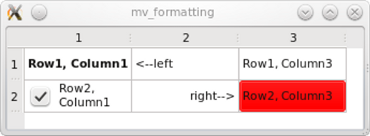
\includegraphics[width=0.5\textwidth]{readonlytable_role}
\end{figure}

实际上,除了 data() 方法外,无需更改其他任何内容即可设置字体,背景色,对齐方式和复选框。
下面是产生上面所示结果的 data() 方法。不同之处在于,这次我们使用参数 int 角色根据其值返回不同的信息。

(文件: examples/widgets/tutorials/modelview/2\_formatting/mymodel.cpp)

\begin{cppcode}
// mymodel.cpp
QVariant MyModel::data(const QModelIndex &index, int role) const
{
    int row = index.row();
    int col = index.column();
    // generate a log message when this method gets called
    qDebug() << QString("row %1, col%2, role %3")
            .arg(row).arg(col).arg(role);

    switch (role) {
    case Qt::DisplayRole:
        if (row == 0 && col == 1) return QString("<--left");
        if (row == 1 && col == 1) return QString("right-->");

        return QString("Row%1, Column%2")
                .arg(row + 1)
                .arg(col +1);
    case Qt::FontRole:
        if (row == 0 && col == 0) { //change font only for cell(0,0)
            QFont boldFont;
            boldFont.setBold(true);
            return boldFont;
        }
        break;
    case Qt::BackgroundRole:
        if (row == 1 && col == 2)  //change background only for cell(1,2)
            return QBrush(Qt::red);
        break;
    case Qt::TextAlignmentRole:
        if (row == 1 && col == 1) //change text alignment only for cell(1,1)
            return Qt::AlignRight + Qt::AlignVCenter;
        break;
    case Qt::CheckStateRole:
        if (row == 1 && col == 0) //add a checkbox to cell(1,0)
            return Qt::Checked;
        break;
    }
    return QVariant();
}
\end{cppcode}

每个格式化属性将通过对 data() 方法的单独调用从模型中请求。
角色参数用于让模型知道请求哪个属性:

\begin{tabular}{|l|m{15em}|l|}
	\hline
	枚举 enum Qt::ItemDataRole & 意义 &类型 \\
	\hline
	Qt::DisplayRole	 & 文本	 &QString \\
	\hline
	Qt::FontRole	& 字体	&QFont\\ 
	\hline
	BackgroundRole &	单元格背景的画笔	& QBrush\\ 
	\hline
	Qt::TextAlignmentRole	& 文本对齐方式 &enum Qt::AlignmentFlag \\
	\hline 
	Qt::CheckStateRole &	使用 QVariant() 取消复选框,使用 Qt::Checked 或 Qt::UnChecked 设置复选框 &	enum Qt::ItemDataRole \\
	\hline
\end{tabular}

请参阅 Qt 明明控件文档了解有关 Qt::ItemDataRole 枚举功能的更多信息。

现在我们需要确定使用分离的模型如何影响应用程序的性能,因此让我们跟踪视图调用 data() 方法的频率。
为了跟踪视图调用模型的频率,我们在 data() 方法中放置了一条调试语句,该语句记录到错误输出流中。
在我们的小示例中,data() 将被调用 42 次。
每次将光标悬停在该字段上时,都会再次调用 data(),每个单元格7次。
这就是为什么在调用 data() 和缓存昂贵的查找操作时确保数据可用的重要原因。

\subsection{表内的时钟}

\begin{figure}[hbt!]  
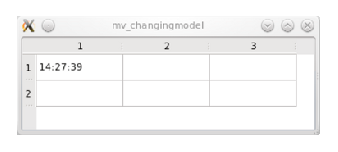
\includegraphics[width=0.5\textwidth]{clock}
\end{figure}

我们仍然使用一个只读表,但是这次内容每秒更改一次,因为我们正在显示当前时间。

(文件:examples/widgets/tutorials/modelview/3\_changingmodel/mymodel.cpp)

\begin{cppcode}
QVariant MyModel::data(const QModelIndex &index, int role) const
{
    int row = index.row();
    int col = index.column();

    if (role == Qt::DisplayRole && row == 0 && col == 0)
        return QTime::currentTime().toString();

    return QVariant();
}
\end{cppcode}

缺少一些东西来使时钟滴答作响。我们需要每秒告诉视图时间已更改,并且需要再次读取。
我们用一个计时器来做到这一点。
在构造函数中,我们将其间隔设置为1秒,然后连接其超时信号。

(文件:examples/widgets/tutorials/modelview/3\_changingmodel/mymodel.cpp)

\begin{cppcode}
MyModel::MyModel(QObject *parent)
    : QAbstractTableModel(parent)
    , timer(new QTimer(this))
{
    timer->setInterval(1000);
    connect(timer, &QTimer::timeout , this, &MyModel::timerHit);
    timer->start();
}
\end{cppcode}

(文件:examples/widgets/tutorials/modelview/3\_changingmodel/mymodel.cpp)

槽函数:

\begin{cppcode}
void MyModel::timerHit()
{
    //we identify the top left cell
    QModelIndex topLeft = createIndex(0,0);
    //emit a signal to make the view reread identified data
    emit dataChanged(topLeft, topLeft, {Qt::DisplayRole});
}
\end{cppcode}

我们通过发射 dataChanged() 信号要求视图再次读取左上角单元格中的数据。
请注意,我们没有将 dataChanged 信号显式连接到视图。这在我们调用 setModel 时自动发生。

\subsection{设置行和列的标题} 

标题可以通过调用视图的一个方法被隐藏: tableView->verticalHeader()->hide();

\begin{figure}[hbt!]  
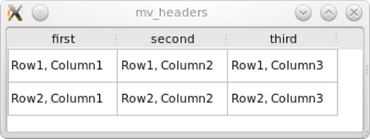
\includegraphics[width=0.5\textwidth]{modelview-header}
\end{figure}

但是,标题内容是通过模型设置的,因此我们重新实现 headerData() 方法:

(文件:examples/widgets/tutorials/modelview/4\_headers/mymodel.cpp)

\begin{cppcode}
QVariant MyModel::headerData(int section, Qt::Orientation orientation, int role) const
{
    if (role == Qt::DisplayRole && orientation == Qt::Horizontal) {
        switch (section) {
        case 0:
            return QString("first");
        case 1:
            return QString("second");
        case 2:
            return QString("third");
        }
    }
    return QVariant();
}
\end{cppcode}

\begin{lstlisting}
方法 headerData() 也具有角色参数,该角色与 MyModel::data() 中的含义相同。
\end{lstlisting}

\subsection{最小编辑示例}

在此示例中,我们将构建一个应用程序,该应用程序通过重复输入表单元格中的值来自动用内容填充窗口标题。为了能够轻松访问窗口标题,我们将 QTableView 放在 QMainWindow 中。

该模型决定编辑功能是否可用。我们仅需修改模型即可启用可用的编辑功能。这可以通过重新实现以下虚函数来完成:setData() 和 flags()。

(文件:examples/widgets/tutorials/modelview/5\_edit/mymodel.h)


\begin{cppcode}
// mymodel.h
#include <QAbstractTableModel>
#include <QString>

const int COLS= 3;
const int ROWS= 2;

class MyModel : public QAbstractTableModel
{
    Q_OBJECT
public:
    MyModel(QObject *parent = nullptr);
    int rowCount(const QModelIndex &parent = QModelIndex()) const override;
    int columnCount(const QModelIndex &parent = QModelIndex()) const override;
    QVariant data(const QModelIndex &index, int role = Qt::DisplayRole) const override;
    bool setData(const QModelIndex &index, const QVariant &value, int role = Qt::EditRole) override;
    Qt::ItemFlags flags(const QModelIndex &index) const override;
private:
    QString m_gridData[ROWS][COLS];  //holds text entered into QTableView
signals:
    void editCompleted(const QString &);
};
\end{cppcode}

我们使用二维数组 QString m\_gridData 来存储我们的数据。这使 m\_gridData 成为 MyModel 的核心。
MyModel 的其余部分就像包装器一样,将 m\_gridData 调整为 QAbstractItemModel 接口。
我们还引入了 editCompleted() 信号,这使得将修改后的文本传输到窗口标题成为可能。

(文件:examples/widgets/tutorials/modelview/5\_edit/mymodel.cpp)

\begin{cppcode}
bool MyModel::setData(const QModelIndex &index, const QVariant &value, int role)
{
    if (role == Qt::EditRole) {
        if (!checkIndex(index))
            return false;
        //save value from editor to member m_gridData
        m_gridData[index.row()][index.column()] = value.toString();
        //for presentation purposes only: build and emit a joined string
        QString result;
        for (int row = 0; row < ROWS; row++) {
            for (int col= 0; col < COLS; col++)
                result += m_gridData[row][col] + ' ';
        }
        emit editCompleted(result);
        return true;
    }
    return false;
}
\end{cppcode}
    
每次用户编辑单元格时都会调用 setData() 。index 参数告诉我们哪个字段已被编辑,value 提供了编辑过程的结果。
该角色将始终设置为 Qt::EditRole,因为我们的单元格仅包含文本。
如果存在一个复选框,并且将用户权限设置为允许选中该复选框,则还将以角色设置为 Qt::CheckStateRole 进行调用。

(文件:\hl{examples/widgets/tutorials/modelview/5\_edit/mymodel.cpp})

\begin{cppcode}
Qt::ItemFlags MyModel::flags(const QModelIndex &index) const
{
    return Qt::ItemIsEditable | QAbstractTableModel::flags(index);
}
\end{cppcode}

单元格的各种属性可以使用 flags() 进行调整。

返回 Qt::ItemIsSelectable | Qt::ItemIsEditable | Qt::ItemIsEnabled 足以显示一个可被单元格选中的编辑器。

如果编辑一个单元格所修改的数据多于该特定单元格中的数据,则该模型必须发射 dataChanged() 信号,以便读取已更改的数据。

\section{中间主题}

\subsection{树视图}

您可以将上面的示例转换为具有树视图的应用程序。
只需将 QTableView 替换为 QTreeView,这将生成一个读/写树。不必对模型进行任何更改。
树不会有任何层次结构,因为模型本身没有任何层次结构。

\begin{figure}[hbt!]  
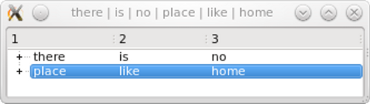
\includegraphics[width=0.5\textwidth]{dummy_tree}
\end{figure}


QListView,QTableView 和 QTreeView 均使用了合并了列表、表和树的模型抽象。
这样就可以让不同类型的视图类使用同一模型。

\begin{figure}[hbt!]  
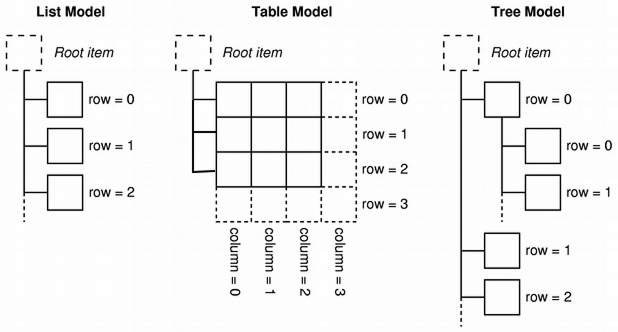
\includegraphics[width=0.5\textwidth]{list_table_tree}
\end{figure}

到目前为止,我们在示例中使用的模型都是这样子的:

\begin{figure}[hbt!]  
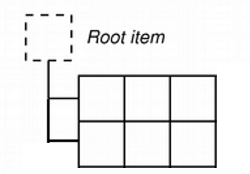
\includegraphics[width=0.5\textwidth]{example_model}
\end{figure}

我们想呈现一棵真正的树。在上面的示例中包装了数据,以建立模型。这次我们使用 QStandardItemModel ,这是用于具有层次结构的数据的容器,也实现了 QAbstractItemModel。
要显示树,必须用 QStandardItem 填充 QStandardItemModelQStandardItem 可以保存项目的所有标准属性,例如文本,字体,复选框或笔刷。

\begin{figure}[hbt!]  
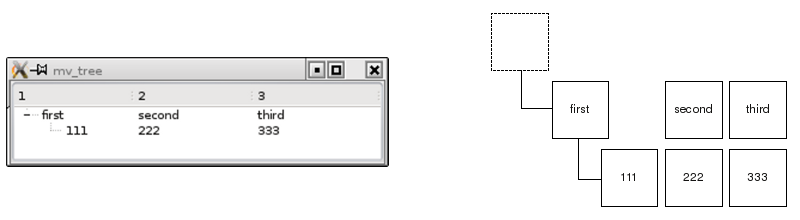
\includegraphics[width=0.5\textwidth]{tree_2_with_algorithm}
\end{figure}

(文件:\hl{examples/widgets/tutorials/modelview/6\_treeview/mainwindow.cpp})

\begin{cppcode}
// modelview.cpp
#include "mainwindow.h"

#include <QTreeView>
#include <QStandardItemModel>
#include <QStandardItem>

MainWindow::MainWindow(QWidget *parent)
    : QMainWindow(parent)
    , treeView(new QTreeView(this))
    , standardModel(new QStandardItemModel(this))
{
    setCentralWidget(treeView);

    QList<QStandardItem *> preparedRow = prepareRow("first", "second", "third");
    QStandardItem *item = standardModel->invisibleRootItem();
    // adding a row to the invisible root item produces a root element
    item->appendRow(preparedRow);

    QList<QStandardItem *> secondRow = prepareRow("111", "222", "333");
    // adding a row to an item starts a subtree
    preparedRow.first()->appendRow(secondRow);

    treeView->setModel(standardModel);
    treeView->expandAll();
}

QList<QStandardItem *> MainWindow::prepareRow(const QString &first,
                                              const QString &second,
                                              const QString &third) const
{
    return {new QStandardItem(first),
            new QStandardItem(second),
            new QStandardItem(third)};
}
\end{cppcode}

我们只需实例化一个 QStandardItemModel 并向构造函数添加几个 QStandardItem。
然后,我们可以建立分层数据结构,因为 QStandardItem 可以容纳其他 QStandardItem。节点在视图内折叠并展开。

\subsection{处理选择}

我们希望访问所选项目的内容,以便将其与层次结构级别一起输出到窗口标题中。

\begin{figure}[hbt!]  
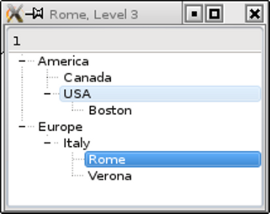
\includegraphics[width=0.5\textwidth]{selection2}
\end{figure}

因此,让我们来创建几个项:

(文件: \hl{examples/widgets/tutorials/modelview/7\_selections/mainwindow.cpp})

\begin{cppcode}
#include "mainwindow.h"

#include <QTreeView>
#include <QStandardItemModel>
#include <QItemSelectionModel>

MainWindow::MainWindow(QWidget *parent)
    : QMainWindow(parent)
    , treeView(new QTreeView(this))
    , standardModel(new QStandardItemModel(this))
{
    setCentralWidget(treeView);
    QStandardItem *rootNode = standardModel->invisibleRootItem();

    //defining a couple of items
    QStandardItem *americaItem = new QStandardItem("America");
    QStandardItem *mexicoItem =  new QStandardItem("Canada");
    QStandardItem *usaItem =     new QStandardItem("USA");
    QStandardItem *bostonItem =  new QStandardItem("Boston");
    QStandardItem *europeItem =  new QStandardItem("Europe");
    QStandardItem *italyItem =   new QStandardItem("Italy");
    QStandardItem *romeItem =    new QStandardItem("Rome");
    QStandardItem *veronaItem =  new QStandardItem("Verona");

    //building up the hierarchy
    rootNode->    appendRow(americaItem);
    rootNode->    appendRow(europeItem);
    americaItem-> appendRow(mexicoItem);
    americaItem-> appendRow(usaItem);
    usaItem->     appendRow(bostonItem);
    europeItem->  appendRow(italyItem);
    italyItem->   appendRow(romeItem);
    italyItem->   appendRow(veronaItem);

    //register the model
    treeView->setModel(standardModel);
    treeView->expandAll();

    //selection changes shall trigger a slot
    QItemSelectionModel *selectionModel = treeView->selectionModel();
    connect(selectionModel, &QItemSelectionModel::selectionChanged,
            this, &MainWindow::selectionChangedSlot);
}
\end{cppcode}

视图在单独的选择模型中管理选择,可以使用 selectionModel() 方法进行检索。我们检索选择模型,以便将槽函数连接到其 selectionChanged() 信号。

(文件: \hl{examples/widgets/tutorials/modelview/7\_selections/mainwindow.cpp})

\begin{cppcode}
void MainWindow::selectionChangedSlot(const QItemSelection & /*newSelection*/, const QItemSelection & /*oldSelection*/)
{
    //get the text of the selected item
    const QModelIndex index = treeView->selectionModel()->currentIndex();
    QString selectedText = index.data(Qt::DisplayRole).toString();
    //find out the hierarchy level of the selected item
    int hierarchyLevel = 1;
    QModelIndex seekRoot = index;
    while (seekRoot.parent() != QModelIndex()) {
        seekRoot = seekRoot.parent();
        hierarchyLevel++;
    }
    QString showString = QString("%1, Level %2").arg(selectedText)
                         .arg(hierarchyLevel);
    setWindowTitle(showString);
}
\end{cppcode}

我们通过调用 treeView->selectionModel()->currentIndex() 来获得与选择相对应的模型索引,并通过使用模型索引来获取字段的字符串。
然后我们只计算项目的hierarchyLevel。顶级项没有父级,并且 parent() 方法将返回默认构造的 QModelIndex()。这就是为什么我们在迭代计算期间使用 parent() 方法迭代到最高级别的原因。

可以检索选择模型(如上所示),但也可以使用 QAbstractItemView::setSelectionModel 进行设置。
这样就可以拥有3个具有同步选择的视图类,因为仅使用了一个选择模型实例。要在3个视图之间共享选择模型,请使用 selectionModel() 并通过 setSelectionModel 将结果分配给第二个和第三个视图类。

\subsection{预定义模型}

使用模型/视图的典型方法是包装特定数据以使其可用于视图类。
但是,Qt 还为常见的底层数据结构提供了预定义的模型。
如果可用的数据结构之一适合您的应用程序,那么预定义的模型可能是一个不错的选择。

\begin{longtable}{|l|l|}
\hline
QStringListModel &	存储字符串列表 \\ 
\hline
QStandardItemModel &	存储任意分层结构的项目\\
\hline
QFileSystemModel
QDirModel	 & 封装本地文件系统\\ 
\hline
QSqlQueryModel &	封装 SQL 结果集\\
\hline
QSqlTableModel	& 封装 SQL 表\\
\hline
QSqlRelationalTableModel &	封装带外键的 SQL 表 \\
\hline
QSortFilterProxyModel	& 排序或者过滤其他模型 \\
\hline
\end{longtable}

\subsection{委托}

到目前为止,在所有示例中,数据均以文本或复选框形式显示在单元格中,并以文本或复选框的形式进行编辑。
提供这些表示和编辑服务的组件称为委托。我们只是刚刚开始使用委托,因为视图使用了默认委托。
但是,假设我们想要一个不同的编辑器(例如,一个滑块或一个下拉列表),或者想象我们想要将数据显示为图形。
让我们看一个名为 Star Delegate 的示例,其中的星星用于显示等级:


\begin{figure}[hbt!]  
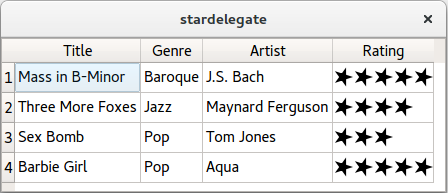
\includegraphics[width=0.5\textwidth]{stardelegate}
\end{figure}

该视图具有 setItemDelegate() 方法,该方法将替换默认委托并安装自定义委托。
可以通过创建从 QStyledItemDelegate 继承的类来编写新的委托。为了编写一个显示星星但没有输入功能的委托,我们只需要重写2个方法即可。


\begin{cppcode}
class StarDelegate : public QStyledItemDelegate
{
    Q_OBJECT
public:
    StarDelegate(QWidget *parent = 0);
    void paint(QPainter *painter, const QStyleOptionViewItem &option,
               const QModelIndex &index) const;
    QSize sizeHint(const QStyleOptionViewItem &option,
                   const QModelIndex &index) const;
};
\end{cppcode}

paint() 根据底层数据的内容绘制星形。可以通过调用 index.data() 查找数据。委托的 sizeHint() 方法用于获取每个星星的尺寸,因此该单元格将提供足够的高度和宽度来容纳星星。

如果要在视图类的网格内以自定义图形显示数据,则编写自定义委托是正确的选择。如果要离开网格,则可以不使用自定义委托,而使用自定义视图类。

Qt 文档中关于委托的其他参考:

\begin{compactitem}
\item Spin Box Delegate Example
\item QAbstractItemDelegate Class Reference
\item QSqlRelationalDelegate Class Reference
\item QStyledItemDelegate Class Reference
\item QItemDelegate Class Reference
\end{compactitem}

\subsection{使用 ModelTest 调试}

模型的被动性质为程序员带来了新的挑战。模型中的不一致会导致应用程序崩溃。
由于该模型会被视图中调用无数次,因此很难找出哪个调用使应用程序崩溃了,以及哪个操作导致了该问题。

Qt Labs 提供了一个名为 ModelTest 的软件,该软件可在您的程序运行时检查模型。
每次更改模型时,ModelTest 都会扫描模型并使用断言报告错误。这对于树模型尤其重要,因为它们的层次结构性质即使是细微的不一致也会留下许多可能性。

与视图类不同,ModelTest 使用超出范围的索引来测试模型。
这意味着您的应用程序可能会因 ModelTest 而崩溃,即使没有它也可以完美运行。因此,在使用 ModelTest 时,您还需要处理所有超出范围的索引。

\section{附录}
\subsection{书籍}

模型/视图编程在 Qt 文档中有相当广泛的介绍,但也有好几本好书。

\begin{compactitem}
\item C++ GUI Programming with Qt 4 / Jasmin Blanchette, Mark Summerfield, Prentice Hall, 2nd edition, ISBN 0-13-235416-0. 
      Also available in German: C++ GUI Programmierung mit Qt 4: Die offizielle Einführung, Addison-Wesley, ISBN 3-827327-29-6
\item The Book of Qt4, The Art of Building Qt Applications / Daniel Molkentin, Open Source Press, ISBN 1-59327-147-6. 
      Translated from Qt 4, Einführung in die Applikationsentwicklung, Open Source Press, ISBN 3-937514-12-0.
\item Foundations of Qt Development / Johan Thelin, Apress, ISBN 1-59059-831-8.
\item Advanced Qt Programming / Mark Summerfield, Prentice Hall, ISBN 0-321-63590-6. 
      This book covers Model/View programming on more than 150 pages.
\end{compactitem}

以下列表概述了上面列出的前三本书中包含的示例程序。
其中一些为开发类似应用程序提供了非常好的模板。

\begin{longtable}{|m{15em}|l|l|l|m{15em}|}
\hline
示例名称 &	使用的视图类	&使用的模型&	涵盖的方面  \\ 
\hline	
Team Leaders &	QListview	&QStringListModel	&	&Book 1, Chapter 10, Figure 10.6 \\
\hline	
Directory Viewer	&QTreeView	&QDirModel	&	&Book 1, Chapter 10, Figure 10.7\\
\hline	
Color Names	 & QListView &	应用于 QStringListModel 的 QSortFilterProxyModel &&		Book 1, Chapter 10, Figure 10.8 \\
\hline	
Currencies &	QTableView &	基于 QAbstractTableModel 的自定义模型 &	只读 	&Book 1, Chapter 10, Figure 10.10  \\ 
\hline
Cities  &	QTableView &	基于 QAbstractTableModel 的自定义模型 &	读/写	&Book 1, Chapter 10, Figure 10.12 \\ 
\hline
Boolean Parser &	QTreeView	& 基于 QAbstractTableModel 的自定义模型	 & 只读 	&Book 1, Chapter 10, Figure 10.14 \\ 
\hline
Track Editor &	QTableWidget &	& 	自定义的委托并提供了自定义的编辑器  &	Book 1, Chapter 10, Figure 10.15 \\ 
\hline
Four directory views &	QListView QTableView QTreeView &	QDirModel	& 演示使用多个视图	&Book2, Chapter 8.2 \\ 
\hline
Address Book &	QListView QTableView QTreeView	& 基于 QAbstractTableModel 的自定义模型& 	读/写 &	Book2, Chapter 8.4 \\
\hline
Address Book with sorting  &		& QSortfilterProxyModel &	引入排序和过滤功能 &	Book2, Chapter 8.5 \\ 
\hline
Address Book with checkboxes &	& &		在模型/视图中引入复选框	 &Book2, Chapter 8.6 \\ 
\hline
Address Book with transposed grid	&	基于 QAbstractProxyModel 的自定义代理模型	& 引入自定义模型 &	Book2, Chapter 8.7 \\ 
\hline
Address Book with drag and drop		& &	引入托拖放支持	& Book2, Chapter 8.8 \\ 
\hline
Address Book with custom editor	&	&	引入自定义委托	& Book2, Chapter 8.9 \\
\hline
Views	& QListView QTableView QTreeView &	QStandardItemModel	& 只读	& Book 3, Chapter 5, figure 5-3 \\ 
\hline
Bardelegate	& QTableView	& &	演示基于 QAbstractItemDelegate 的自定义委托	& Book 3, Chapter 5, figure 5-5 \\ 
\hline
Editdelegate &	QTableView	& &		基于 QAbstractItemDelegate 的用于编辑的自定义委托	&Book 3, Chapter 5, figure 5-6 \\ 
\hline
Singleitemview	& 基于 QAbstractItemView 的自定义视图	&&	自定义视图	&Book 3, Chapter 5, figure 5-7 \\ 
\hline
listmodel &	QTableView	&基于 QAbstractTableModel 的自定义模型	&只读&	Book 3, Chapter 5, Figure 5-8 \\ 
\hline
treemodel	& QTreeView	& 基于 QAbstractTableModel 的自定义模型	&只读	&Book 3, Chapter 5, Figure 5-10 \\ 
\hline
edit integers &	[QListView]	& 基于 QAbstractTableModel 的自定义模型	 & 读/写	& Book 3, Chapter 5, Listing 5-37, Figure 5-11 \\ 
\hline
sorting	 & QTableView	& 应用于 QStringListModel 的 QSortFilterProxyModel	& 演示排序	& Book 3, Chapter 5, Figure 5-12 \\ 
\hline
\end{longtable}

\subsection{Qt 文档}

Qt5.0提供了19个模型/视图示例。这些示例可以在 项目视图示例 页面上找到。


\begin{longtable}{|l|m{10em}|m{10em}|l|}
\hline
示例名称	& 使用的视图类	& 使用的模型 & 	涵盖的方面  \\ 
\hline
Address Book &	QTableView &QAbstractTableModel QSortFilterProxyModel &	使用QSortFilterProxyModel从一个数据池生成不同的子集 \\ 
\hline
Basic Sort/Filter Model	& QTreeView &	QStandardItemModel QSortFilterProxyModel & 	 \\ 
\hline
Chart	& 自定义视图	& QStandardItemModel	& 设计与选择模型协作的自定义视图 \\ 
\hline
Color Editor Factory &	QTableWidget	&&	扩展一个带有新的自定义的编辑器的委托来选择颜色 \\ 
\hline
Combo Widget Mapper &使用 [QDataWidgetMapper] () 映射 QLineEdit、QTextEdit 和 QComboBox	 & QStandardItemModel	& 演示了QComboBox如何作为视图类 \\ 
\hline
Custom Sort/Filter Model &	QTreeView &	QStandardItemModel QSortFilterProxyModel &	子类化 QSortFilterProxyModel 用于高级排序和过滤 \\ 
\hline
Dir View &	QTreeView &	QFileSystemModel &	演示如何将模型指定给视图的非常小的示例 \\ 
\hline
Editable Tree Model	 &QTreeView	 &自定义树模型	& 使用树的综合示例,演示了如何使用底层自定义模型编辑单元格和树结构 \\ 
\hline
Fetch More&	QListView	&自定义列表模型 &	动态变化的模型 \\ 
\hline
Frozen Column &	QTableView	& QStandardItemModel	& \\ 
\hline
Interview &	Multiple	 & 自定义项目模型 &	多个视图 \\ 
\hline
Pixelator	& QTableView	& 自定义表模型	& 实现一个自定义委托 \\ 
\hline
Puzzle	& QListView	& 自定义列表模型 &	支持拖放的模型/视图 \\ 
\hline
Simple DOM Model&	QTreeView	 & 自定义树模型 &	自定义的只读的树模型的示例 \\ 
\hline
Simple Tree Model	 & QTreeView	& 自定义树模型	& 自定义的只读的树模型的示例 \\ 
\hline
Simple Widget Mapper&	使用 QDataWidgetMapper 映射 QLineEdit、QTextEdit 和 QSpinBox&	QStandardItemModel &	QDataWidgetMapper 的基本用法 \\ 
\hline
Spin Box Delegate & 	QTableView &	QStandardItemModel &	使用旋转框作为单元格编辑器的自定义委托 \\ 
\hline 
Spreadsheet	& QTableView	 &&	自定义委托  \\ 
\hline 
Star Delegate &	QTableWidget	&&	功能齐全的自定义委托示例 \\ 
\hline
\end{longtable}

还提供了模型/视图技术的参考文档。